\documentclass{beamer}
%
% Choose how your presentation looks.
%
% For more themes, color themes and font themes, see:
% http://deic.uab.es/~iblanes/beamer_gallery/index_by_theme.html
%
\mode<presentation>
{
  \usetheme{default}      % or try Darmstadt, Madrid, Warsaw, ...
  \usecolortheme{default} % or try albatross, beaver, crane, ...
  \usefonttheme{default}  % or try serif, structurebold, ...
  \setbeamertemplate{navigation symbols}{}
  \setbeamertemplate{caption}[numbered]
} 

\usepackage[utf8x]{inputenc}
\usepackage{float}
\usepackage[spanish]{babel}
\usepackage{graphicx}
\usepackage{multirow}
\usepackage{parskip}
\usepackage{pst-all, color}
\usepackage[T1]{fontenc}
%algorithm
\usepackage{algpseudocode}
\usepackage{algorithm}

\title[GIT]{Git and Git Flow}
\author{Camilo Andrés Rodríguez Garzón}
\institute{Universidad EAFIT}
\date{\today}

\begin{document}

\begin{frame}
  \titlepage
\end{frame}

% Uncomment these lines for an automatically generated outline.
\begin{frame}{Contenido}
  \tableofcontents
\end{frame}

\section{What is Git?}

\begin{frame}{What is Git?}
\begin{itemize}
\item Started \textbf{2005}
\item Created for \textbf{(Linus Torvalds)}
\item Git is a free and open source distributed \textbf{version control system}
\end{itemize}

\end{frame}

\section{Some commands}

\begin{frame}{Some commands}

\begin{block}{when you begin a new project}
\begin{itemize}
\item git clone url -- downloads branch global in git local
\item git fecth -- if you need to change to other branch		
\item git checkout 
\end{itemize}
\end{block}

\begin{block}{when you work in a common day}
\begin{itemize}
\item git status -- show you local changes
\item git pull origin name-branch 					
\item git add name-file --	add all current changes for the next commit
\item git commit -m "information of state" --	commit previously staged changes
\item git push origin name-branch --	put changes in global repository
\end{itemize}
\end{block}

\end{frame}

\section{}
\begin{frame}{Other commands}

\begin{block}{when you require to solve advanced issues}
\begin{itemize}

\item git checkout -b name-new-branch -- create new branch with the same features of the current branch
\item git merge
\item git stash
\item git stash pop
\item git reset
\item git revert
\item git cherrypick
\end{itemize}

\end{block}

\end{frame}

\section{Git flow}
\begin{frame}{Git flow}
El modelo de ramificación \textbf{git flow} de \textbf{Vincent Driessen} es un flujo de trabajo de gestión de lanzamiento y ramificación git que ayuda a los desarrolladores a realizar un seguimiento de las características, revisiones y lanzamientos en proyectos de software.

\end{frame}

\section{Instalación}
\begin{frame}{Instalación}

\begin{figure}[H]
\centering

\includegraphics[width=0.4\textwidth]{github}
\caption{\href{https://github.com/nvie/gitflow/wiki/Installation}{\textbf{\textit{Instalando git-flow}}}}
\end{figure}
\end{frame}

\section{Work flow}
\begin{frame}{Work flow}

\begin{figure}[H]
\centering
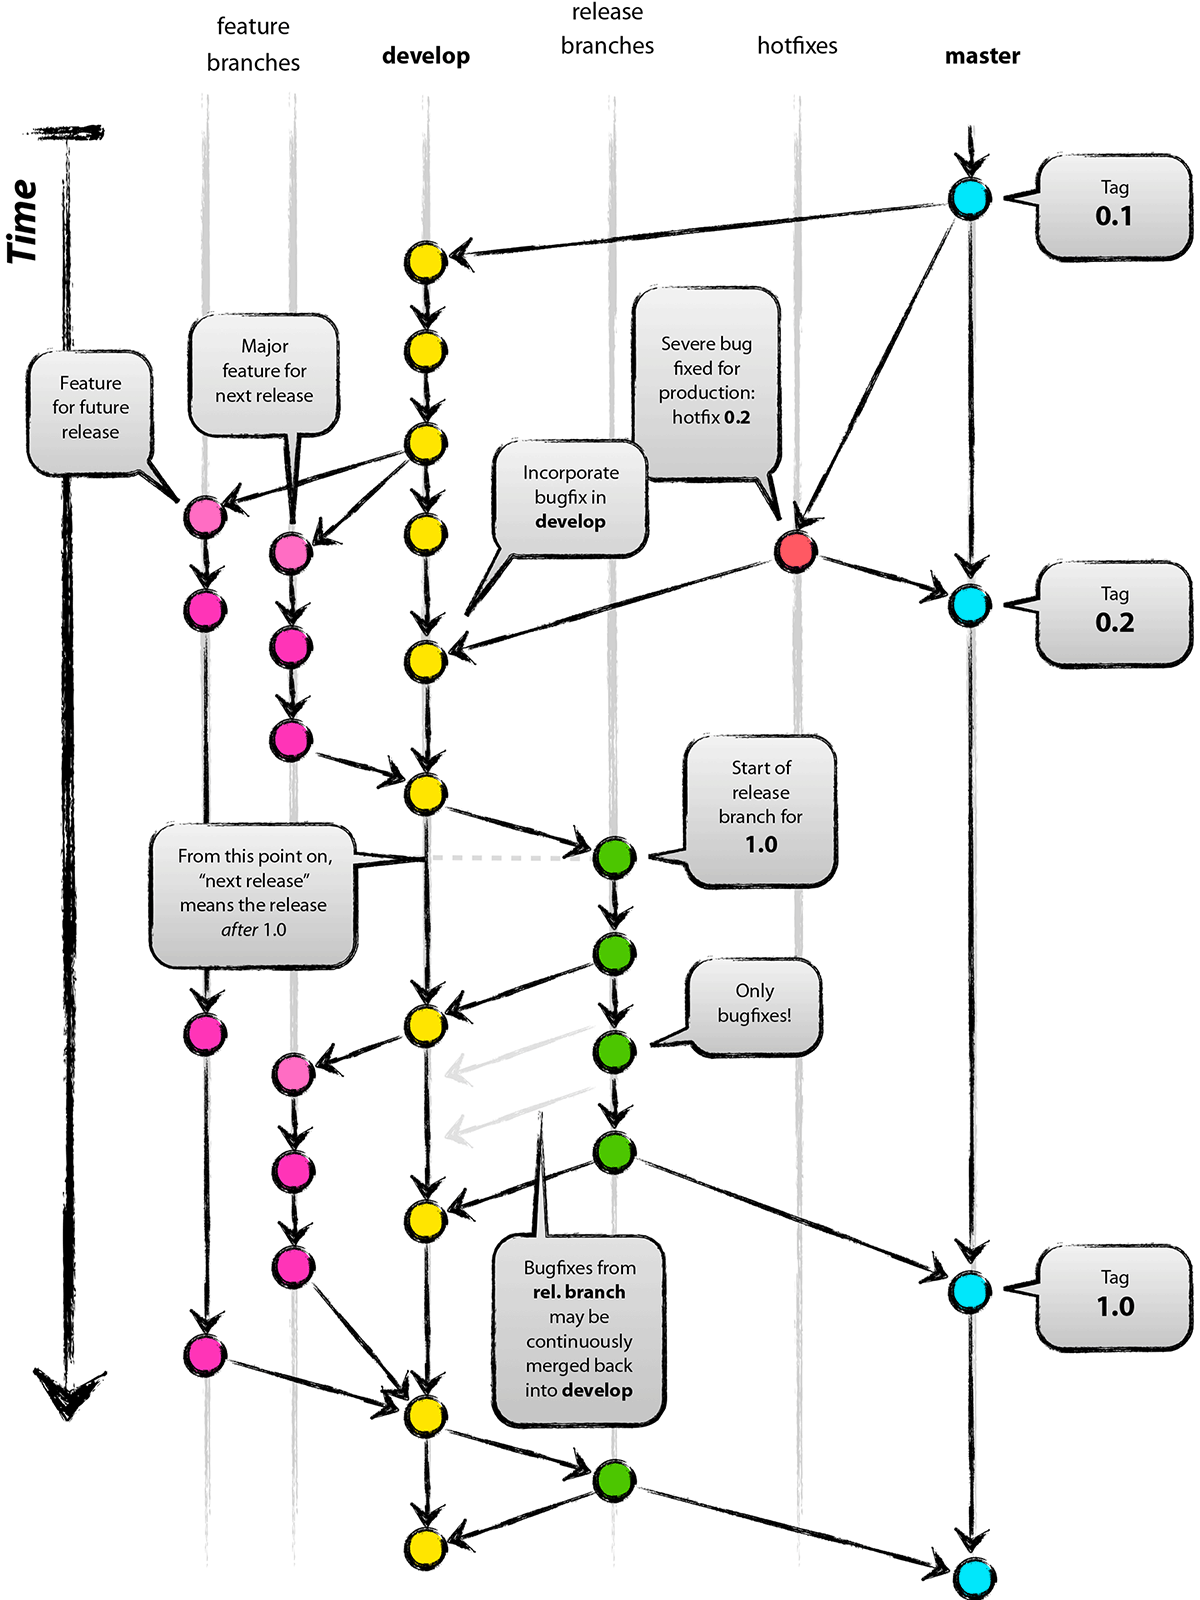
\includegraphics[width=0.6\textwidth]{git-flow.png}
\caption{\label{fig:Figura2} }
\end{figure}

\end{frame}

\section{Inicialización}
\begin{frame}{Inicialización}

Para inicializar un nuevo repositorio con la estructura de rama básica, use:

\begin{itemize}
\item git flow init -d
\end{itemize}

\end{frame}

\section{Feature}
\begin{frame}{Crear feature}

\begin{block}{Para list/start/finish feature branches, usar:}
\begin{itemize}
\item git flow feature
\item git flow feature start <name> [<base>]
\item git flow feature finish <name>
\end{itemize}
\end{block}

\begin{block}{Ejemplo desde el branch feature/CA-006}
git flow feature start CA-007 develop
\end{block}

\end{frame}


\section{}
\begin{frame}{Crear feature}

\begin{block}{Para push/pull una feature branch a el repositorio remoto, usar:}
\begin{itemize}
\item git flow feature publish <name>
\item git flow feature track <name> ó 
\item git flow feature pull <origin> <name>
\end{itemize}
\end{block}

\end{frame}

\section{Release}
\begin{frame}{Crear release}

\begin{block}{Para list/start/finish release branches, usar:}
\begin{itemize}
\item git flow release
\item git flow release start <release> [<base>]
\item git flow release finish <release>
\end{itemize}
\end{block}

\begin{block}{Ejemplo desde el branch feature/CA-007}
git flow release start oca-1.0.0 develop
\end{block}
\end{frame}

\section{Hotfix}
\begin{frame}{Crear hotfix}

\begin{block}{Para list/start/finish hotfix branches, usar:}
\begin{itemize}
\item git flow hotfix
\item git flow hotfix start <release> [<base>]
\item git flow hotfix finish <release>
\end{itemize}
\end{block}

\begin{block}{Ejemplo desde el branch feature/CA-007}
git flow hotfix start oca-007 master
\end{block}
\end{frame}

\section{Bibliografía}
\begin{frame}[allowframebreaks]
    \frametitle{Bibliografía}
    \bibliographystyle{ieeetr}
    \tiny{ 
        \bibliography{ref.bib} \
        \
        \nocite{*}}
\end{frame}

\begin{frame}
\begin{center}
\textbf{Gracias...}
\end{center}
\end{frame}

\begin{frame}{Como funciona Git flow}
\href{https://vimeo.com/16018419}{Un ejemplo de como funciona esto}
\end{frame}
\end{document}
